\documentclass[serif,9pt]{beamer}
\usepackage{color,listings}
\usepackage{ragged2e}
\usepackage[spanish]{babel}
\usepackage[utf8]{inputenc}
\usepackage{graphicx}

\definecolor{dkgreen}{rgb}{0,0.6,0}
\definecolor{gray}{rgb}{0.5,0.5,0.5}
\definecolor{mauve}{rgb}{0.58,0,0.82}
\definecolor{lgray}{rgb}{0.99,0.97,0.95}
\newcommand{\X}{\textbf{X}}
\newcommand{\Y}{\textbf{Y}}
\newcommand{\Z}{\textbf{Z}}
\newcommand{\G}{\textbf{G}}
\newcommand{\R}{\textbf{R}}
\newcommand{\V}{\textbf{V}}
\newcommand{\Q}{\textbf{Q}}
\newcommand{\h}{\textbf{H}}
\newcommand{\T}{\textbf{T}}

\def\E{\mathbb{E}}
\def\C{\mathbb{C}}
\def\N{\mathbb{N}}

\setbeamercovered{transparent}


\usetheme{Frankfurt}
%\usecolortheme{rose}
%\usecolortheme{lily}
\usepackage{amsmath, multirow}
%\usepackage{color, amsmath, wrapfig, anysize, graphicx, hyperref, amsthm, fancyhdr, amssymb,geometry,amsfonts,float}

\newcommand{\ds}{\displaystyle}


\titlegraphic{
\includegraphics[width=4cm]{utfsm.eps}}%
   %\includegraphics[width=4cm]{fig/inria.eps}}

\begin{document}
\title{Current Investigation\\ Toward a Security Reference Architecture of Web Browser} 
\author[Paulina Silva Ghio]{\textsc{Paulina Silva Ghio} \\ \medskip
\small{}
\medskip
\url{pasilva@alumnos.inf.utfsm.cl}}
\institute[]{}
\date{22-03-2016/23-03-2016.}

\begin{frame}[plain]
\titlepage
\end{frame}


\begin{frame}
\frametitle{Index}
\tableofcontents
\end{frame} 


\section{Introduction}
\subsection{Context}
\begin{frame}
	\frametitle{Context}

	\begin{itemize}
		\item Web Browser's war in the nineties. 
		\item Built and fix.
		\item Web Browser: a tool used daily.
		\item Common user uses its services.
		\item Many type of implementations.
		\item Web 2.0 y 3.0: AJAX (Asynchronous Javascript and XML).
	\end{itemize}
	\begin{figure}[h]
	    \centering
	    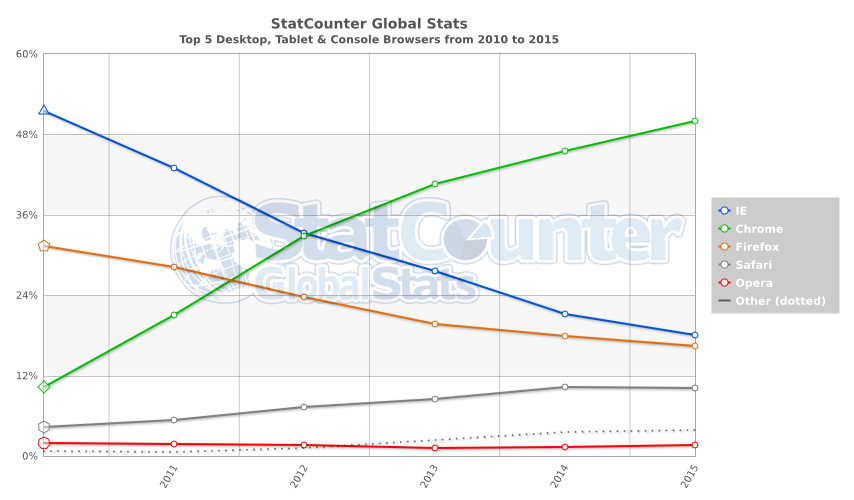
\includegraphics[scale=0.3]{figures/StatCounter-browser-ww-yearly-2010-2015.png}
	    \caption{Market Percentaje of each Browser. Cite: \cite{statBrow}}
	    \label{fig:UsageShare}
	\end{figure}
\end{frame}

% \subsection{Actualidad}
% \begin{frame}
% 	\frametitle{Actualidad}
% 	\begin{itemize}
% 		\item Sistemas actuales son muy complejos.
% 		\item Es necesario utilizar metodologías que aseguren: Requerimientos Funcionales y No-Funcionales.
% 		\item Defectos y errores en el Software generan vulnerabilidades.
% 		\item La Seguridad es un costo ``extra", a veces no considerado.
% 	\end{itemize}
% 	\begin{block}{Las vulnerabilidades...}
% 		Ocurren por que no se ha tomado en cuenta la seguridad en el desarrollo.
% 	\end{block}
% \end{frame}

\subsection{Motivation}
\begin{frame}
	\frametitle{Motivation}
	\onslide{Browser is an indispensable tool, this lets:}
	\begin{itemize}
		\item New ways of interacting.
		\item Lower building costs for a client program.
		\item Already implemented a lot of robust security features in the browser.
		\item Reuse.
	\end{itemize}
	
	\begin{block}<2->{Principal Concerns}
	\begin{itemize}
		\item Systems which are called by users using a browser.
		\item Stakeholders involved: browser's user, host's user and the external service used.
	\end{itemize}
	\end{block}
\end{frame}

\section{Problem}
\subsection{Threats and Vulnerabilities}
\begin{frame}
	\frametitle{Threats and Vulnerabilities}
	\begin{columns}
	\column{0.5\textwidth}
	\begin{minipage}[c][0.4\textheight][c]{\linewidth}
	  \centering
	  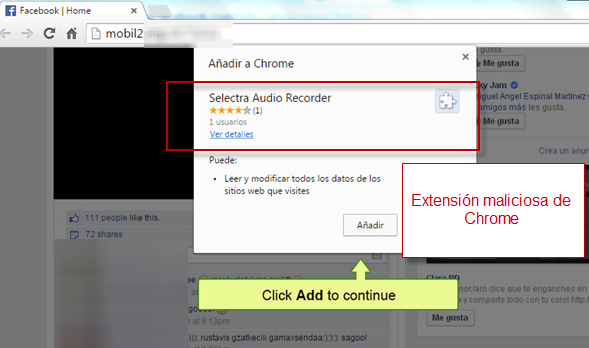
\includegraphics[scale=0.3]{figures/fbporn3.png}
	  \label{fig:Malware}
	\end{minipage}
	\begin{minipage}[c][0.4\textheight][c]{\linewidth}
	  \centering
	  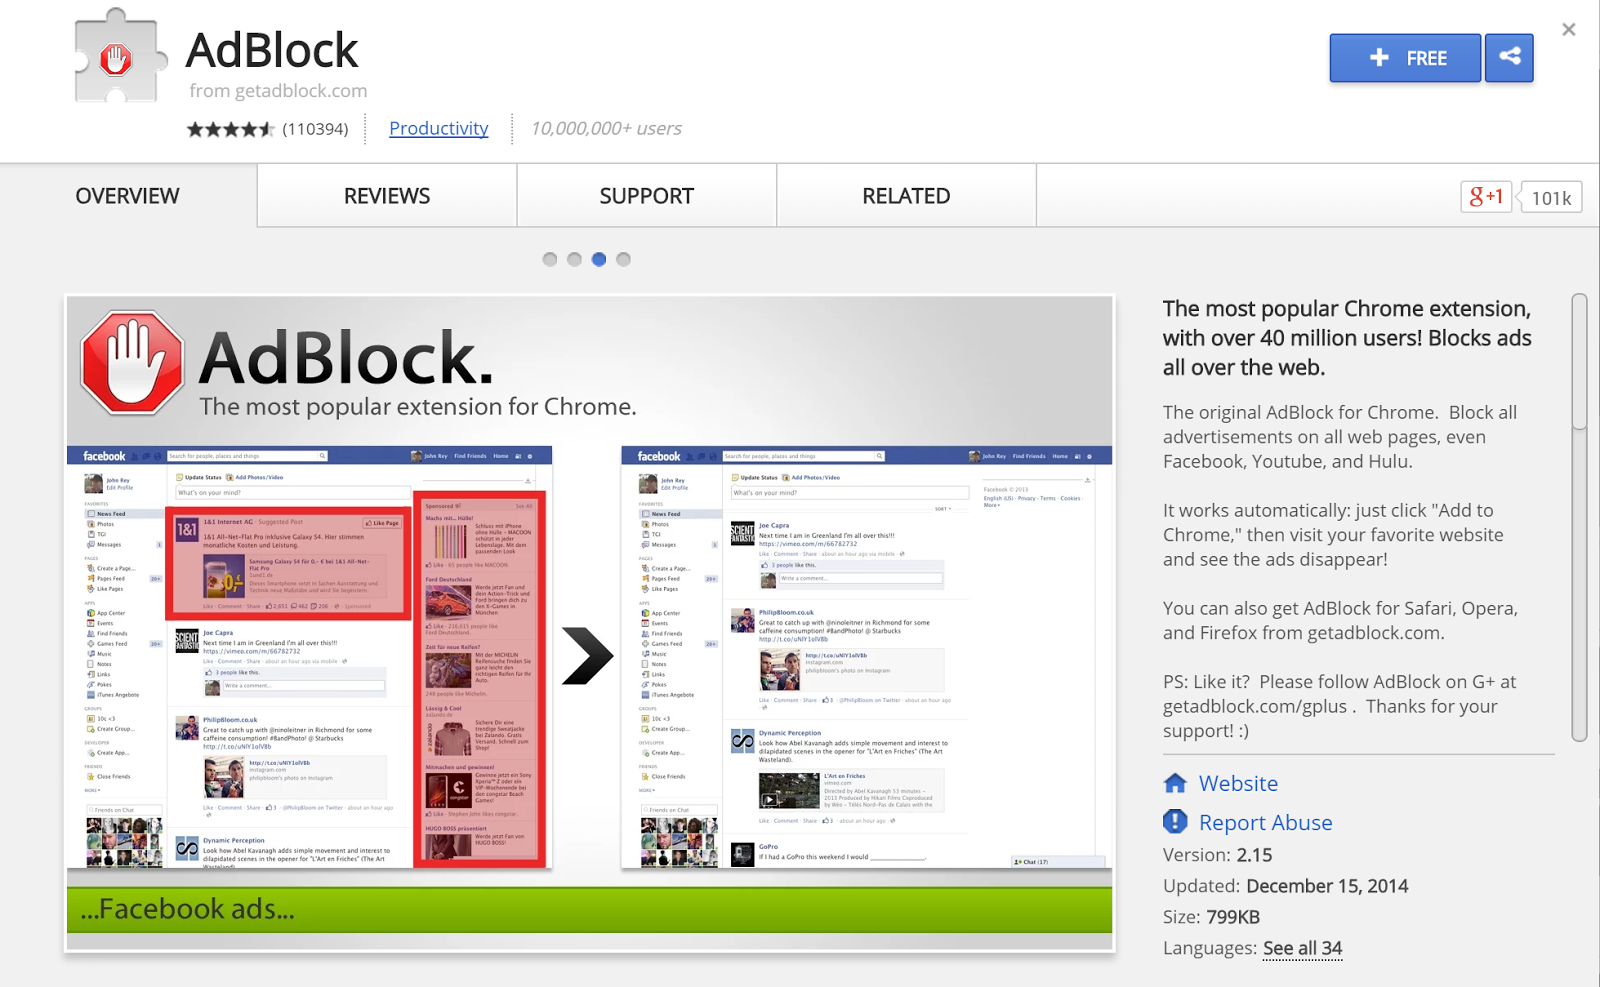
\includegraphics[scale=0.10]{figures/Adblock.png}
	  \label{fig:vulnExt}
	\end{minipage}
	\column{0.5\textwidth}
	\begin{minipage}[c][0.4\textheight][c]{\linewidth}
	  \begin{enumerate}
	  \item Installation of Malware and malicious Extensions.
	  \item Benign-but-buggy Extensions.
	  \item Man in the Browser.
	  \item Code Injection.
	  \end{enumerate}
	\end{minipage}
	\begin{minipage}[c][0.4\textheight][c]{\linewidth}
	  \centering
	  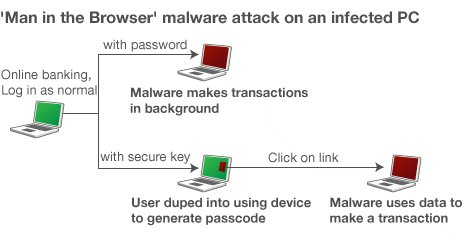
\includegraphics[scale=0.45]{figures/_58291188_malware_464v2.jpg}
	\end{minipage}
	\end{columns}
\end{frame}

\subsection{Problems}
\begin{frame}
	\frametitle{Problems}
	\begin{itemize}
		\item<1-> Lack of knowledge in browser's security aspects, could affect directly the development of applications and stakeholders. 
		\item<2-> Scarce documentation and none unification of concepts. No formal descriptions for browser related concepts.
	\end{itemize}
\end{frame}

\section{Theoretical Framework}
\subsection{Reference Architecture (RA)}
\begin{frame}
	\frametitle{Reference Architecture (RA) for the browser}
		\begin{itemize}
			\item<1> Specifies the decomposition of the systems into subsystems, interactions between these parts and functionality distribution between them.
			\item<1> Captures the essence of the architecture through a collection of similar systems, using architectonic reuse.
			\item<1> Currently, there is no consensus in how to define an RA, what should have and how should be built. We use architectural patterns.
			\item<2> Describes concerns and quality attributes needed.
			\item<2> Helps: developers, in general stakeholders.
			\item<2> Compares design decisions.
			\item<3> Holistic view of the system.
		\end{itemize}
\end{frame}

\subsection{Security Reference Architecture (SRA)}
\begin{frame}
	\frametitle{Security Reference Architecture (SRA)}
	\begin{itemize}
		\item<1> Holistic view of security, taking into account the threats.
		\item<1> Abstraction of defense mechanism described as security patterns.
		\item<2> Unifies terminology.
		\item<2> Can help to evaluate a system and its security requirements.
	\end{itemize}
\end{frame}

\subsection{Misuse Patterns}
\begin{frame}
	\frametitle{Misuse Patterns}
	\begin{itemize}
		\item<1> Describes from the point of view of the attacker, how an attack can be done (which units uses and how), analizes the ways of stopping the attack by enumerating the possible security patterns that could be used, and describes how to trace back the attack once it has occured (recolection of forensic data).
		\item<2> Let teach and communicate possible ways how a system can be misused.
	\end{itemize}
\end{frame}


\subsection{State of Art}
\begin{frame}
	\frametitle{State of Art}
	\begin{itemize}
		\item<1-> Have not found updated works about Reference Architectures of the Browser. The work of Grosskurth et al. \cite{preprint-grosskurth-browser-archevol} is close, but the technique is different.
		\item<1-> Works: 
		\begin{itemize}
			\item<2> Larrondo et al. \cite{535061}: analyzes the browser and obtains a Domain Model,  an Object Model, a Feature Tree which describes structure and functionality of the browser.
			\item<3> Grosskurth et al. \cite{2005-grosskurth-browser-refarch,preprint-grosskurth-browser-archevol}: Reverse engineering tool to obtain a high-level architecture of open-source browsers: Mozilla y Konqueror.
			\item<4> Godfrey et al. \cite{Godfrey2000}: similar to the above but only for Mozilla, and also obtained architectural views of the system.
			\item<5> Lwin \cite{Lwin2009}]: proposes a browser called Anfel SOFT, with AI to improve user's experience.
		\end{itemize}
		\item<6-> Scarse and poor documentation. None unification of concepts.
		\item<7-> As for a SRA, thre was no work found.
	\end{itemize}
\end{frame}


\section{Proposal}
\subsection{General and specific objectives/goals}
\begin{frame}
	\frametitle{General and specific objectives/goals}
	\begin{block}{General objective}
		\begin{small}
		\begin{itemize}
			\item Build an organized body of information about the Web Browser and its security.
			\item Systematize, organize and classify adquiered knowledge in a document, with a semi-formal format.
			\item Better comprehension of browser's security.
		\end{itemize}
		\end{small}
	\end{block}
	\begin{block}<2->{Specific objectives}
		\begin{small}
			\begin{itemize}
				\item A guide to comunicate relevant concepts.
				\item Improve our Reference Architecture and continue our misuse pattern catalog. 
				\item Build a conceptual model of browser's security, a Security Reference Architecture.
				\item Get to know how social engineering can affect the browser.
				\item Use Experimental Software Engineering techniques.
			\end{itemize}
		\end{small}
	\end{block}
\end{frame}


\subsection{Hypotesis}
\begin{frame}
	\frametitle{Hypotesis}	
	\begin{block}{Main Hypotesis}
			H1: The definition of a Security Reference Architecture for the Web Browser allows to abstract and capture main structural aspects, its behavior and security related requirements.
	\end{block}
	% \begin{block}{Otra posible hipótesis}
	% 	%\begin{itemize}
	% 	H2: El uso de una Arquitectura de Referencia de Seguridad permite añadir seguridad al desarrollo de aplicaciones web.
	% 		%\item H3: El uso de una Arquitectura de Referencia de Seguridad permite la construcción de Browser Seguros.
	% 	%\end{itemize}
	% \end{block}
\end{frame}

\subsection{Validation}
\begin{frame}
	\frametitle{Validation}	
	\begin{itemize}
	\item<1> Reference Architecture and Security Reference Architecture are not implemented. They are abstract models.
	\item<1> Experts opinions.
	\item<2> *PLoP conferences and ``shepherding" process. Conferences: AsianPLoP y EuroPLoP.
	\item<2> Experimental Software Engineering to validate or reject hypotesis. 
	\end{itemize}
\end{frame}

\subsection{Work already done}
\begin{frame}
	\frametitle{Work already done}
	\begin{itemize}
		\item RA and misuse pattern.
		\item AsianPLoP and EuroPLoP.
	\end{itemize}
\end{frame}

\section{Side work}
\begin{frame}
	\frametitle{Side work}
	\begin{itemize}
		\item<1-> Fondecyt Project: Software Development Initiatives to Identify and Mitigate Security Threats -- A Systematic Mapping.
			\begin{itemize}
				\item<2> A systematic mapping has been conducted to cover the existent technologies for identification and mitigation of security threats.
				\item<3> A total of 10 different techniques covering threats identification and 8 covering the mitigation of threats were found. 
				\item<4> All the initiatives were integrated to at least one activity of the Software Development Lifecycle (SDLC), while 7 show signs of being adopted in the industry. 
				\item<5> The mapping found only 15 studies that covered 11 different iniatiatives. 
				\item<6> Only two techniques presented scientific evidence of its results through controlled experiments, while others selected studies presented informal case studies or examples.
			\end{itemize}
		\item<7-> Fondecyt Project: Research
			\begin{itemize}
				\item<8> A Theoretical Framework for quality assessment of security metrics.
				\item<9> How to evaluate security in software development
			\end{itemize}
	\end{itemize}
\end{frame}


\begin{frame}
	\frametitle{Questions?}
	¡Muchas Gracias!, Thank you!, Arigatou Gozaimashita!, Grazie!
\end{frame}

\bibliography{refTodas}
\bibliographystyle{IEEEtran}

\end{document}

